
\begin{frame}{Appendix --- Voter Behavior: Turnout by Voter Profile}
\hypertarget{src:turnoutprofile}{}
\small
Compulsory turnout is mechanically frozen, but turnout among the \textbf{facultative} electorate (ages 16--17 and 70$+$) is free to move (it rose from \TurnoutRateTwenty\% to \TurnoutRateFortyFour\% overall, with far larger municipal swings), and turnout has a strong \textbf{education gradient}. If litigation demobilizes, these elastic margins are where it should show. Each dot is the 2SLS effect of a one-SD shock; bars are 90\% (thick) and weak-IV (tF, thin) intervals. From the TSE \emph{perfil do eleitorado}; state FE, clustered by state.
\smallskip
\begin{center}
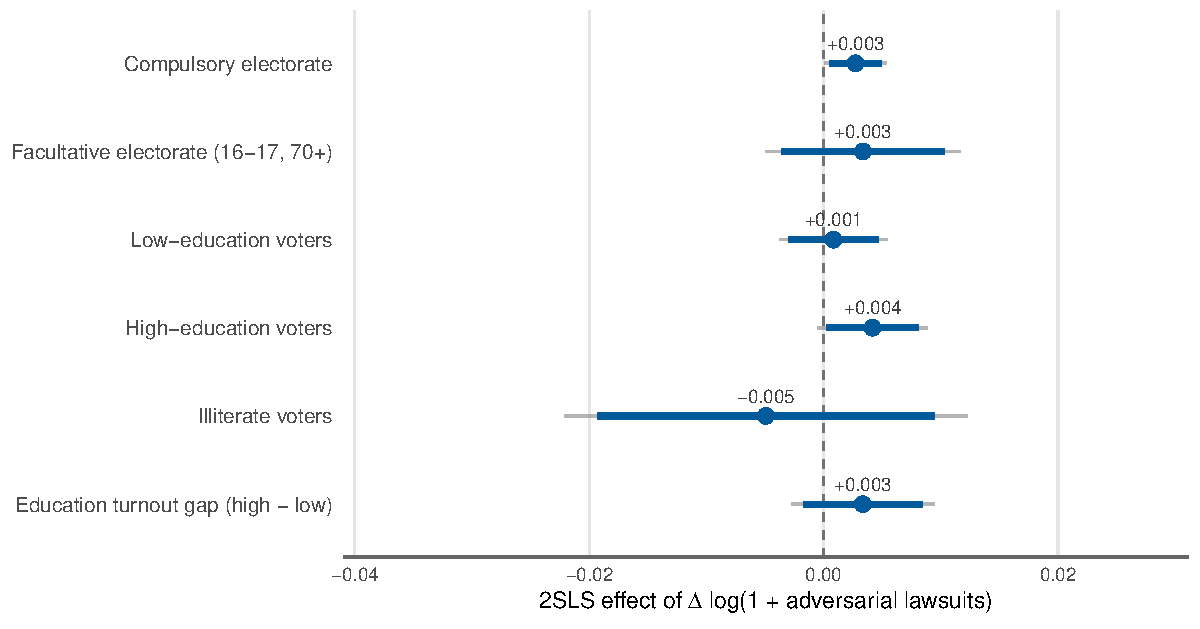
\includegraphics[width=\linewidth,height=0.48\textheight,keepaspectratio]{../figures/turnout_coefplot.pdf}
\end{center}
\smallskip
\footnotesize \textbf{Null on every margin.} Every interval crosses zero and the magnitudes are negligible: a one-SD rise in judicialization ($\approx\TreatSDMult\times$ more litigation) moves facultative turnout by only $\FacultativePerSDSigned$~pp and the education gap by $\EduGapPerSDSigned$~pp, both indistinguishable from zero. The high-education margin is closest to a signal ($p=\HighEdP$) but does not clear conventional significance.\hfill\hyperlink{app:turnoutprofile}{\beamergotobutton{Full table}}
\end{frame}
